\subsection{Sonja Lehmann}

\begin{wrapfigure}{L}{0.35\textwidth}
  \vspace{-20pt}
  \begin{center}
    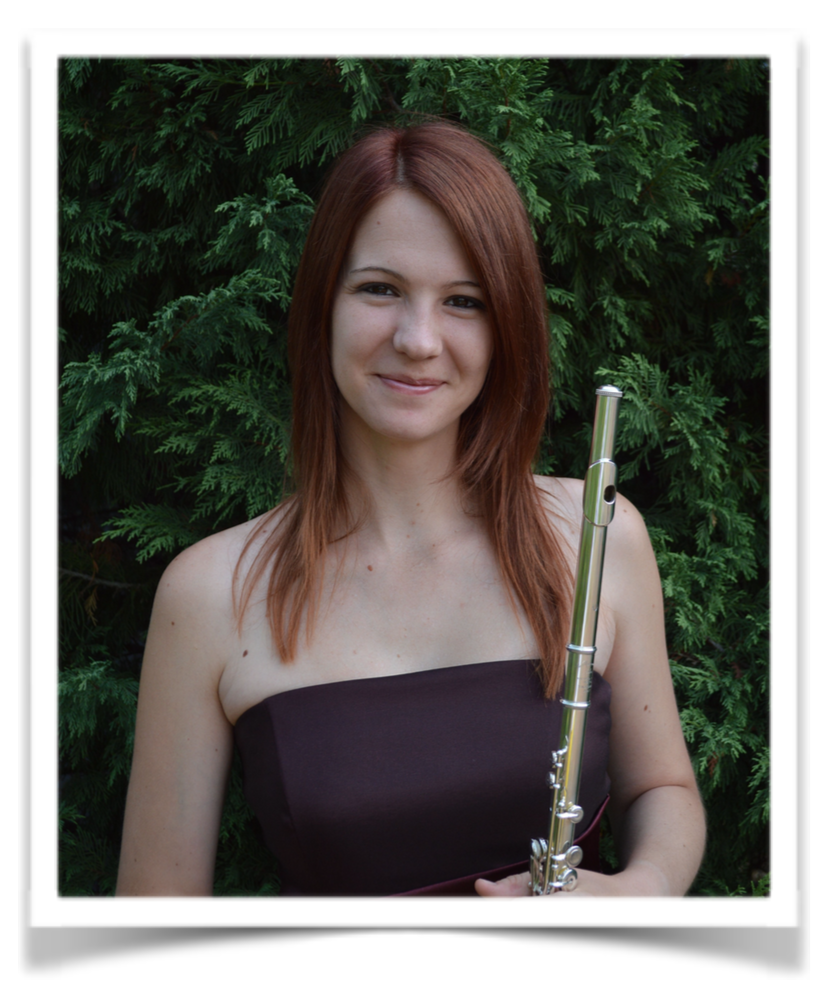
\includegraphics[width=0.32\textwidth]{./images/Sonja_Lehmann}
  \end{center}
  \vspace{-40pt}
\end{wrapfigure}


\textbf{Name:} Sonja Lehmann

\textbf{Alter:} 19

\textbf{Studium:} Kunst \and Deutsch auf Lehramt, 2. Semester

\textbf{Computerkenntnisse:} Wenig

\textbf{Interessen:} Reiten, Lesen, Querflöte spielen

\textbf{Vorlieben/Qualifkationen:} Sehr kompetent in Word, Excel, Powerpoint\\Handy/PC wird primär für produktive Arbeit benutzt\\Ist nicht viel im sozialen Netzwerk unterwegs

\textbf{Motivation:} Interessiert sich für \texttt{ArguMens}, da sie mit der App die Möglichkeit bekommt, durch gute Argumente auf sich Aufmerksam zu machen. Sonja erwartet eine einfache Bedienung.




\subsection{Xiao Lee}

\begin{wrapfigure}{L}{0.4\textwidth}
  \vspace{-20pt}
  \begin{center}
    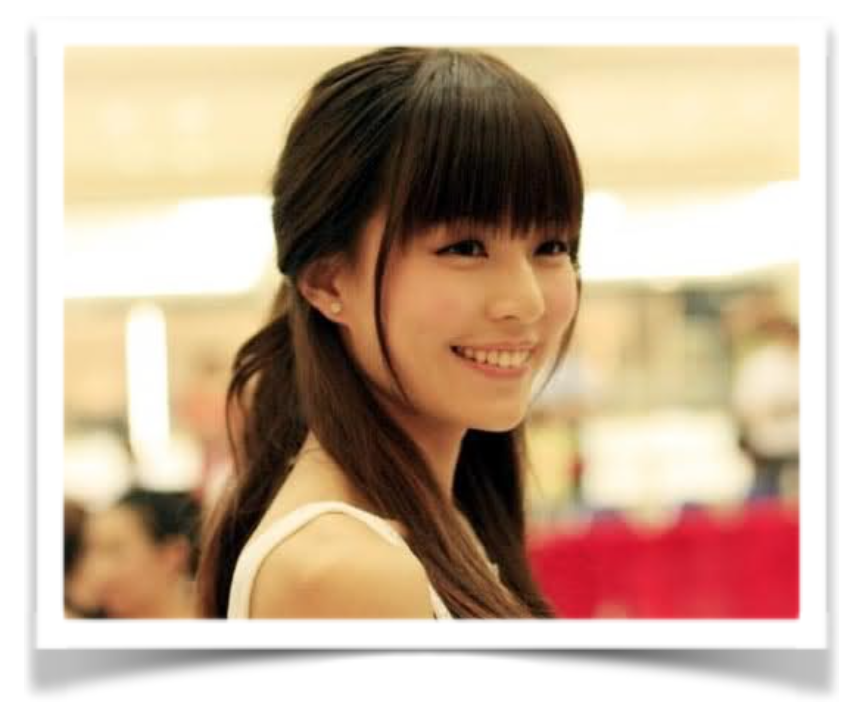
\includegraphics[width=0.38\textwidth]{./images/Xiao_Lee}
  \end{center}
  \vspace{-40pt}
\end{wrapfigure}


\textbf{Name:} Xiao Lee

\textbf{Alter:} 22

\textbf{Studium:} Maschinenbau, Master

\textbf{Besonderes:} Studiert mit Stipendium in Deutschland

\textbf{Computerkenntnisse:} Moderat

\textbf{Interessen:} Engagiert sich im AStA, Macht Judo, Fotografiert gerne

\textbf{Vorlieben:} Kennt professionelle Anwendungen \and Office, Nutzt soziale Netzwerke, Funktionalität ist ihr wichtiger, als Ästhetik

\textbf{Motivation:} Interessiert sich für \texttt{ArguMens}, um sich im Falle eines hohen Funktionsumfangs mit dem Tool zu beschäftigen und sich besser in der Vorlesung zu engagieren. Eine schnelle Bedienung ist ihr wichtig. Die App muss für Xiao einen Nutzen erfüllen.



\subsection{Torben Bruhns}

\begin{wrapfigure}{L}{0.35\textwidth}
  \vspace{-20pt}
  \begin{center}
    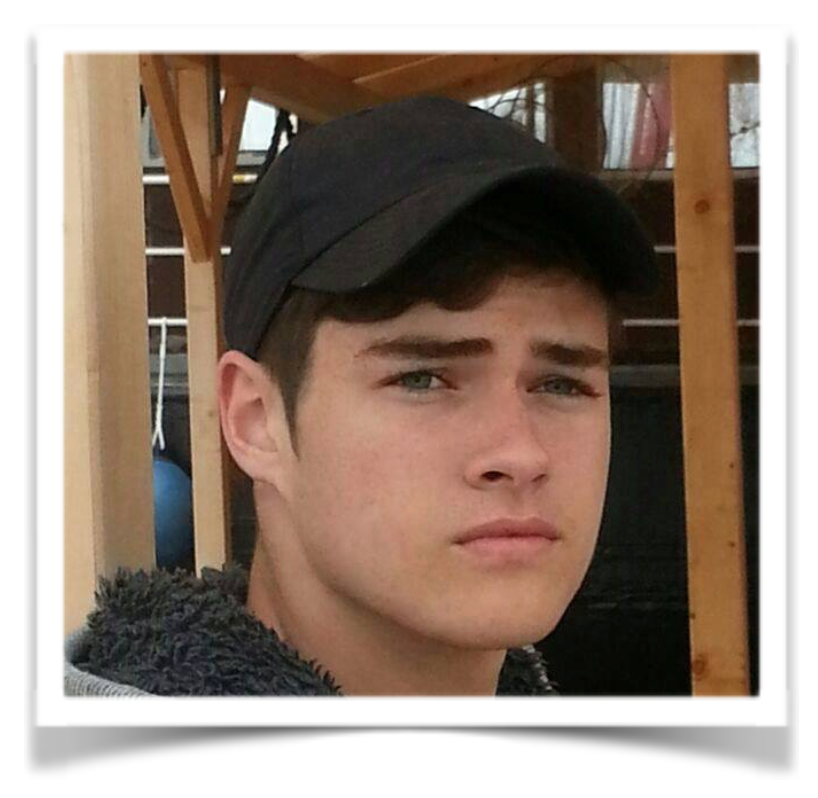
\includegraphics[width=0.32\textwidth]{./images/Torben_Bruhns}
  \end{center}
  \vspace{-40pt}
\end{wrapfigure}

\textbf{Name:} Torben Bruhns

\textbf{Alter:} 27

\textbf{Studium:} Informatik, 6. Semester

\textbf{Computerkenntnisse:} Sehr gut

\textbf{Ziele:} Bachelor- Abschluss schaffen durch so wenig Aufwand wie möglich 

\textbf{Vorlieben:} Computerspiele, Soziale Netzwerke, Aktive Benutzung komplizierter IDEs, Serien

\textbf{Motivation:} Interessiert sich für \texttt{ArguMens}, um den Dozenten fälschlicherweise von nicht existierendem Engangement zu überzeugen (Vortäuschen von aktiver Beteiligung).



\subsection{Mathias Kunz}

\begin{wrapfigure}{L}{0.45\textwidth}
  \vspace{-20pt}
  \begin{center}
    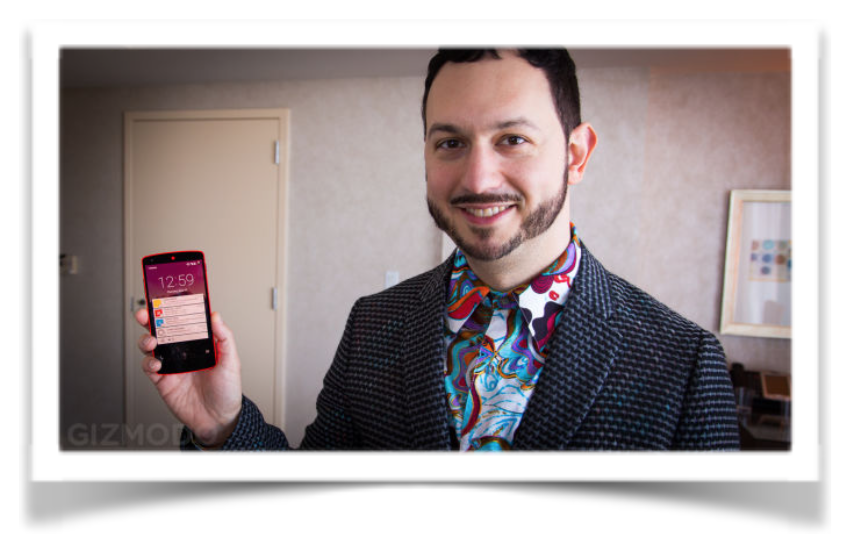
\includegraphics[width=0.42\textwidth]{./images/Mathias_Kunz}
  \end{center}
  \vspace{-40pt}
\end{wrapfigure}


\textbf{Name:} Mathias Kunz

\textbf{Alter:} 48

\textbf{Beruf:} Designer, Dozent für Kunst \and Design

\textbf{Familienstand:} Ledig

\textbf{Interessen:} Kochen, Malen, Wein, Magazine für Technik \and Design

\textbf{Vorlieben:} Ästhetik $\rightarrow$ MacOS, Moderne
 Designtrends, Benutzt Adobe Programme \and WebApps



\textbf{Motivation:} Interessiert sich für \texttt{ArguMens}, da er durch die App seine Vorlesung interaktiv gestalten kann. Die Integration von Studenten liegt ihm sehr am Herzen. Mathias wünscht sich, dass Studenten durch die App lernen, andere Standpunkte zu betrachten. Er erwartet ein modernes und intuitives Design.



\subsection{Francois Carton}

\begin{wrapfigure}{L}{0.35\textwidth}
  \vspace{-20pt}
  \begin{center}
    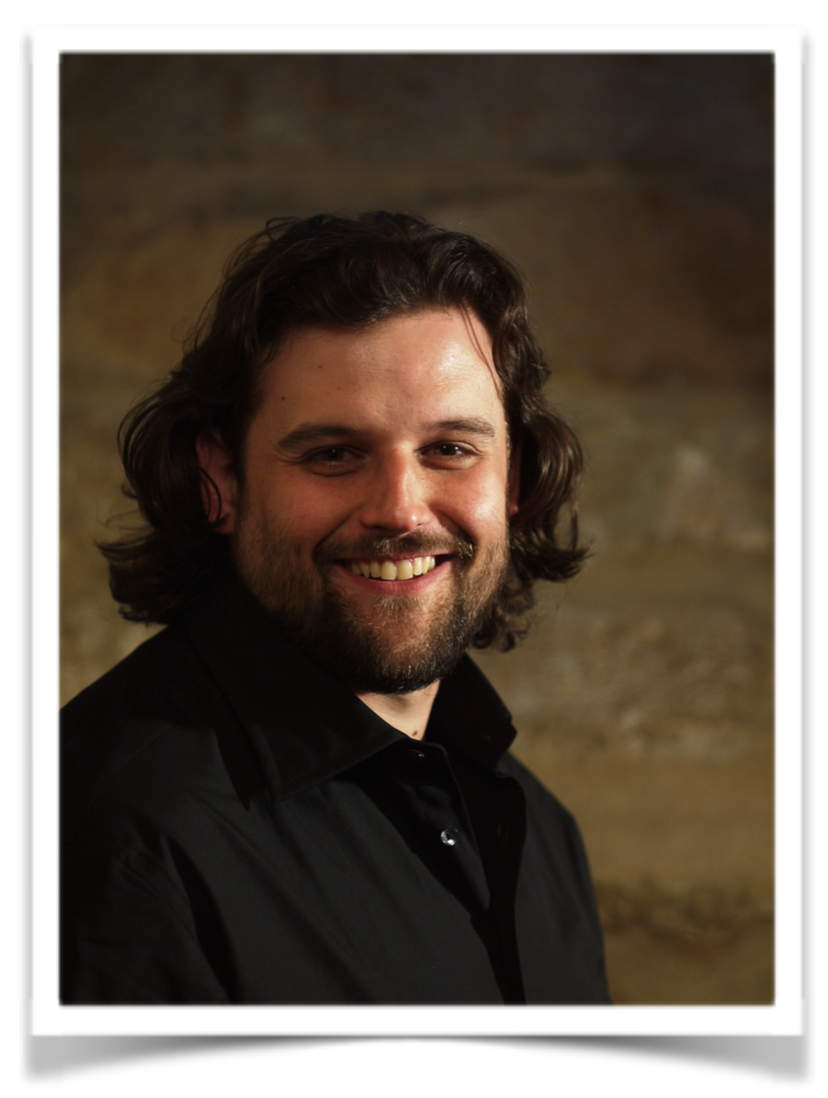
\includegraphics[width=0.32\textwidth]{./images/Francois_Carton}
  \end{center}
  \vspace{-40pt}
\end{wrapfigure}


\textbf{Name:} Francois Carton

\textbf{Alter:} 49

\textbf{Beruf:} Dozent für Mathematik \and Philosophie in Lyon

\textbf{Besonderes:} Eingefleischter Franzose

\textbf{Ziele:} Kennt Computer noch aus der DOS-Zeit.\\
Benutzt spezielle/professionelle Software.\\ 
Bevorzugt Tastenkombinationen und hat keine Ahnung von Ästhetik

\textbf{Vorlieben:} Computerspiele, Soziale Netzwerke, Aktive Benutzung komplizierter IDEs, Serien

\textbf{Motivation:} Interessiert sich für \texttt{ArguMens}, um mit den Studenten eine intensive Diskussion führen zu können. Der Fokus soll hierbei auf dem Inhalt liegen. Schnelle aber auch komplexe Einordnung der Argumente ist erwünscht (Gewichtung der Relevanz bzw. Filterung von Irrelevanz).
